\documentclass[11pt]{standalone}
\usepackage{tikz}
\usetikzlibrary{shapes.geometric}
\usetikzlibrary{arrows.meta,calc,decorations.pathmorphing,shapes.geometric,backgrounds,plotmarks,shapes.multipart}
\begin{document} 
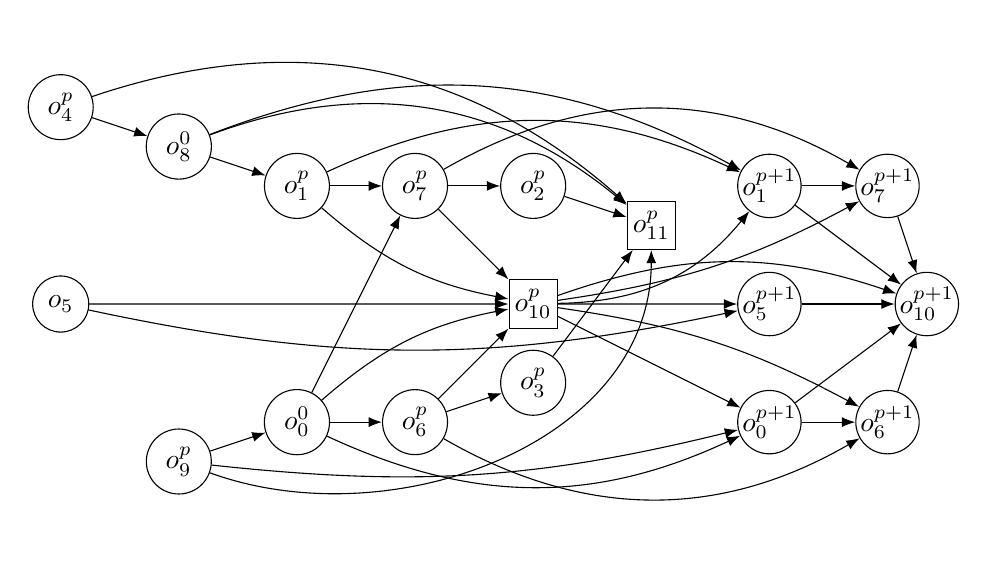
\begin{tikzpicture}

\begin{scope}[framed,local bounding box=scope1,node distance=1.5cm,every node/.style={circle,draw},square/.style={regular polygon,regular polygon sides=4,inner sep=-.5}]
% Nodes
\node[] (o5) {$o_5$};
\node[above of = o5,yshift=1cm] (o4) {$o_4^p$};
\node[right of = o4,yshift=-.5cm] (o8) {$o_8^0$};
\node[right of = o8,yshift=-.5cm] (o1) {$o_1^p$};
\node[right of = o1] (o7) {$o_7^p$};
\node[right of = o7] (o2) {$o_2^p$};
\node[square,right of = o2,yshift=-.5cm] (o11) {$o_{11}^p$};
\node[square,below of = o2] (o10) {$o_{10}^p$};
\node[below of = o10,yshift=.5cm] (o3) {$o_3^p$};
\node[left of = o3,yshift=-.5cm] (o6) {$o_6^p$};
\node[left of = o6] (o0) {$o_0^0$};
\node[left of = o0,yshift=-.5cm] (o9) {$o_9^p$};

\node[right of = o11,yshift=.5cm,inner sep=0] (o1_1) {$o_1^{p+1}$};
\node[below of = o1_1,inner sep=0] (o5_1) {$o_5^{p+1}$};
\node[below of = o5_1,inner sep=0] (o0_1) {$o_0^{p+1}$};
\node[right of = o1_1,inner sep=0] (o7_1) {$o_7^{p+1}$};
\node[right of = o0_1,inner sep=0] (o6_1) {$o_6^{p+1}$};
\node[right of = o5_1,xshift=.5cm,inner sep=0] (o10_1) {$o_{10}^{p+1}$};

%arcs
\path (o5) edge[-{Latex[]}] (o10);
\path (o4) edge[-{Latex[]}] (o8);
\path (o4) edge[-{Latex[]},bend left=30] (o11);
\path (o8) edge[-{Latex[]}] (o1);
\path (o8) edge[-{Latex[]},bend left=30] (o11);
\path (o1) edge[-{Latex[]}] (o7);
\path (o1) edge[-{Latex[]},bend right=15] (o10);
\path (o7) edge[-{Latex[]}] (o2);
\path (o7) edge[-{Latex[]}] (o10);
\path (o2) edge[-{Latex[]}]  (o11);
\path (o9) edge[-{Latex[]}]  (o0);
\path (o9) edge[-{Latex[]}, out=340,in=270]  (o11);
\path (o0) edge[-{Latex[]}]  (o6);
\path (o0) edge[-{Latex[]},bend left=15]  (o10);
\path (o6) edge[-{Latex[]}]  (o3);
\path (o6) edge[-{Latex[]}]  (o10);
\path (o3) edge[-{Latex[]}]  (o11);
\path (o0) edge[-{Latex[]}]  (o7);

\path (o5_1) edge[-{Latex[]}]  (o10_1);
\path (o6_1) edge[-{Latex[]}]  (o10_1);
\path (o7_1) edge[-{Latex[]}]  (o10_1);
\path (o0_1) edge[-{Latex[]}]  (o10_1);
\path (o1_1) edge[-{Latex[]}]  (o10_1);

\path (o10) edge[-{Latex[]},bend right = 25]  (o1_1);
\path (o1) edge[-{Latex[]},bend left = 25]  (o1_1);
\path (o8) edge[-{Latex[]},bend left = 25]  (o1_1);

\path (o10) edge[-{Latex[]}]  (o5_1);
\path (o5) edge[-{Latex[]},bend right = 12]  (o5_1);

\path (o10) edge[-{Latex[]}]  (o0_1);
\path (o0) edge[-{Latex[]},bend right = 25]  (o0_1);
\path (o9) edge[-{Latex[]},bend right = 10]  (o0_1);

\path (o10) edge[-{Latex[]},bend right = 10]  (o7_1);
\path (o1_1) edge[-{Latex[]}]  (o7_1);
\path (o7) edge[-{Latex[]},bend left = 30]  (o7_1);

\path (o10) edge[-{Latex[]},bend left = 10]  (o6_1);
\path (o0_1) edge[-{Latex[]}]  (o6_1);
\path (o6) edge[-{Latex[]},bend right = 30]  (o6_1);

\path (o10) edge[-{Latex[]},bend left = 19]  (o10_1);

\end{scope}

\end{tikzpicture}
\end{document}